\chapter{Dinámica de Friedmann y ecuación de estado}

\lectureoverview{La expansión homogénea debe distinguirse de la física local de los sistemas ligados, y la geometría intrínseca, de la forma de una inmersión. Una vez establecidas estas distinciones, el principio cosmológico reduce la métrica del espacio-tiempo a un único factor de escala \(a(t)\) y un único índice de curvatura \(k\). La componente temporal de la ecuación de Einstein se convierte entonces en la ecuación de energía de Friedmann. Para resolverla, todavía necesitamos la relación material entre la presión y la densidad de energía. La termodinámica adiabática y la ecuación de estado \(P=w\rho\) dan \(\rho\propto a^{-3(1+w)}\), unificando la materia, la radiación y la energía del vacío en un mismo marco.}

\section{Preguntas que fijan el panorama físico}

\subsection{¿Podría el espacio repetirse antes del horizonte?}

Un universo plano finito puede representarse mediante una celda periódica. Si esa celda fuera más pequeña que la región observable, la luz podría atravesarla y el cielo mostraría imágenes repetidas de las mismas estructuras. Detectar esas repeticiones es más difícil que reconocer simplemente una galaxia familiar: las imágenes llegan desde direcciones y épocas distintas y están alteradas por la evolución cósmica. Aun así, la topología periódica tiene consecuencias observables.

\begin{classroomqa}
\audiencequestion{¿Podría el universo entero ser más pequeño que el universo observable?}
\lecturerresponse{Un toro con identificaciones periódicas es la propuesta natural. En ese caso, observaríamos copias repetidas de la misma región física; en sentido figurado, nos veríamos a nosotros mismos por la puerta trasera. Las búsquedas de la periodicidad cósmica correspondiente no han encontrado indicios que la respalden, aunque sí imponen límites a las celdas fundamentales pequeñas. Esta posibilidad es geométricamente coherente, pero estos indicios no favorecen que el universo sea más pequeño que la región ya observada. \lecturetimestamp{00:01:17--00:02:33}}
\end{classroomqa}

\subsection{La expansión no separa los sistemas ligados}

La expansión cósmica describe el movimiento a gran escala de la materia en movimiento libre dentro de la geometría cosmológica media. No es una orden universal para que toda longitud propia aumente. Las fuerzas electromagnéticas mantienen ligados los átomos, la gravedad mantiene ligados los sistemas planetarios y las fuerzas moleculares ordinarias mantienen ligados los objetos sólidos. En estas escalas, dichas interacciones son enormemente más intensas que la corrección cosmológica.

\begin{classroomqa}
\audiencequestion{¿La energía oscura causa la expansión, y por qué los átomos o las órbitas planetarias no se expanden con el espacio?}
\lecturerresponse{Ya se sabía que el universo se expandía antes de descubrirse la energía oscura. Esta modifica la expansión al acelerarla; no es ni la definición ni la causa original de la expansión. Un sistema ligado no sigue el flujo de Hubble porque predominan sus fuerzas locales. Un fondo acelerado puede producir una perturbación ínfima en un átomo o una órbita, pero las fuerzas de enlace ordinarias restablecen un equilibrio casi inalterado, en vez de permitir que el sistema se desintegre. \lecturetimestamp{00:02:36--00:06:50}}
\end{classroomqa}

\subsection{La energía en una geometría dependiente del tiempo}

La objeción que queda no se refiere a las fuerzas, sino al balance de energía. Si una órbita ligada se opone continuamente a una pequeña perturbación cosmológica, ¿de dónde procede la energía necesaria? La premisa traslada una ley de conservación de un fondo estático a un espacio-tiempo sin simetría global de traslación temporal.

\begin{classroomqa}
\audiencequestion{¿De dónde procede la energía cuando las fuerzas de enlace locales se oponen a la expansión?}
\lecturerresponse{La conservación de la energía en un universo estático se desprende de la invariancia frente a traslaciones temporales: el fondo y sus leyes tienen el mismo aspecto si un experimento se desplaza en el tiempo. Un espacio-tiempo en expansión no es invariante frente a traslaciones temporales en ese sentido global, por lo que no tiene por qué existir una única energía total conservada para el universo entero. La conservación local del tensor de energía-momento sí se mantiene y aparecerá más adelante como la ecuación de continuidad. Lo que falla es la afirmación ingenua de que una energía cósmica definida globalmente debe permanecer constante mientras cambia la geometría. \lecturetimestamp{00:06:52--00:09:24}}
\end{classroomqa}

\subsection{La homogeneidad es una afirmación de grano grueso}

El principio cosmológico depende de la escala. El aire de una habitación cerrada puede ser casi uniforme a escala de la habitación, pero es granular a escala molecular. El universo también contiene planetas, galaxias, cúmulos y fluctuaciones de densidad. La homogeneidad y la isotropía se refieren a su comportamiento promediado en distancias suficientemente grandes para que esas estructuras dejen de privilegiar una posición o dirección.

\begin{classroomqa}
\audiencequestion{¿Las estructuras ligadas a pequeña escala contradicen la homogeneidad y la isotropía?}
\lecturerresponse{No. La homogeneidad exacta falla a pequeña escala, igual que falla para el aire cuando se resuelven las moléculas individuales. A escalas de cientos de millones de años luz o más, la distribución observada es aproximadamente uniforme e independiente de la dirección. Más allá de la región que podemos observar, la homogeneidad sigue siendo una hipótesis cuyas consecuencias deben ponerse a prueba, no un hecho establecido. \lecturetimestamp{00:09:27--00:10:55}}
\end{classroomqa}

\section{La homogeneidad y la isotropía como propiedades métricas}

La homogeneidad y la isotropía son, antes que nada, propiedades geométricas. La ecuación de Einstein nos dirá cómo cambia la geometría con el tiempo. Primero debemos especificar qué tipo de geometría espacial se permite en cada instante.

\begin{classroomqa}
\audiencequestion{¿Qué significan matemáticamente la homogeneidad y la isotropía?}
\lecturerresponse{Describa el espacio mediante una métrica y elija coordenadas \(x^i\) centradas en un punto. Ahora elija coordenadas \(y^i\) centradas en otro punto. La homogeneidad significa que una transformación puede desplazar el origen y dejar la métrica con la misma forma funcional. Así, todos los puntos son geométricamente equivalentes. La isotropía añade simetría rotacional alrededor de cada punto, de modo que ninguna dirección es privilegiada. \lecturetimestamp{00:11:13--00:14:26}}
\end{classroomqa}

\begin{definition}
Un espacio es \emph{homogéneo} si una isometría puede llevar cualquier punto a cualquier otro. Es \emph{isótropo} respecto de un punto si las rotaciones alrededor de él dejan inalterada su geometría. Un espacio homogéneo e isótropo no tiene ni una posición ni una dirección privilegiadas.
\end{definition}

El plano euclídeo hace transparente la definición. En coordenadas cartesianas,
\begin{equation}
ds^2=dx_1^2+dx_2^2.
\label{eq:c04-flat-metric}
\end{equation}
Desplacemos el origen mediante las constantes \(a_1\) y \(a_2\):
\begin{equation}
y_1=x_1+a_1,
\qquad
y_2=x_2+a_2.
\label{eq:c04-flat-translation}
\end{equation}
Como \(dy_i=dx_i\), la métrica transformada es
\begin{equation}
ds^2=dy_1^2+dy_2^2.
\end{equation}
Han cambiado los símbolos usados para etiquetar el punto, pero no la regla para medir distancias. Esta es la realización más sencilla de la homogeneidad. Las rotaciones también preservan la métrica, por lo que el plano es asimismo isótropo.

La esfera es menos trivial solo porque sus coordenadas son menos cómodas. Si se elige el polo sur como origen, la esfera unitaria bidimensional puede escribirse como
\begin{equation}
d\Omega_2^2=dr^2+\sin^2 r\,d\theta^2.
\label{eq:c04-sphere-metric}
\end{equation}
Giremos la esfera de modo que un polo este pase a ser el nuevo origen. La transformación de coordenadas es engorrosa, pero el resultado vuelve a ser la ecuación~\eqref{eq:c04-sphere-metric}. Ningún punto de una esfera redonda es geométricamente distinguible.

\begin{classroomqa}
\audiencequestion{¿Un toro plano con identificaciones periódicas es homogéneo e isótropo?}
\lecturerresponse{Es homogéneo bajo traslaciones: todos los puntos de la celda periódica tienen la misma geometría local. No es completamente isótropo, porque las identificaciones seleccionan direcciones y longitudes periódicas privilegiadas. Mirar a lo largo de uno de esos ejes es globalmente distinto de mirar en una dirección oblicua genérica. Por tanto, el toro es un ejemplo claro de homogeneidad sin isotropía completa. \lecturetimestamp{00:20:18--00:21:30}}
\end{classroomqa}

La uniformidad observada a gran escala motiva el principio cosmológico dentro de nuestro horizonte. Extenderlo más allá de la región observable es un postulado, no una observación directa. Aceptamos ese postulado porque define una geometría precisa cuyas consecuencias pueden contrastarse con los datos.

\section{Geometría intrínseca e inmersión}

Cuando se dice que el espacio es esférico, es tentador imaginar la superficie de goma de un globo situada dentro de una habitación más grande. Esa imagen puede servir para dibujar, pero la habitación circundante no forma parte de la afirmación cosmológica. Lo que importa es la geometría \emph{intrínseca}: consiste en las distancias y los ángulos que pueden medir los observadores que permanecen dentro del espacio.

\subsection{Universos unidimensionales cerrados}

Consideremos un universo unidimensional cerrado. Podemos dibujarlo como un círculo, un cuadrado con esquinas redondeadas o un lazo con forma de cacahuete. Un habitante confinado a la línea solo mide las distancias a lo largo de ella. Si dos lazos tienen la misma longitud total, sus habitantes encuentran la misma geometría intrínseca, aunque los dibujos sean completamente distintos.

\begin{figure}[htbp]
\centering
\includegraphics[width=0.72\textwidth]{lecture_04_figure_05.png}
\caption{Lazos cerrados redondos y deformados, usados para distinguir la geometría intrínseca de la forma de la inmersión. Este fotograma posterior conserva dibujos realizados durante la discusión anterior; el contenido pertinente aparece en 00:23:21--00:25:59.}
\label{fig:c04-intrinsic-board}
\lectureframe{00:59:54.899}
\end{figure}

Toda métrica unidimensional es localmente plana. Un trozo corto de cuerda puede enderezarse sin estirarlo, de modo que la curvatura visible en el plano circundante es extrínseca, no intrínseca. Un lazo cerrado tiene un módulo global, su longitud, pero carece de curvatura local intrínseca que sus habitantes unidimensionales puedan medir.

\begin{figure}[htbp]
\centering
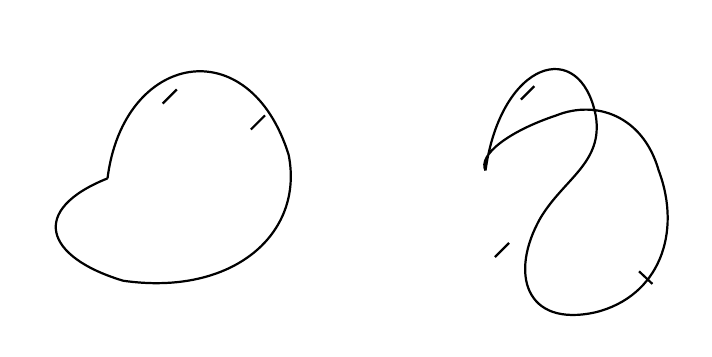
\begin{tikzpicture}[scale=1.0]
\draw[line width=0.8pt] (0,0)
  .. controls (0.2,1.6) and (1.8,1.9) .. (2.3,0.3)
  .. controls (2.5,-0.7) and (1.6,-1.5) .. (0.2,-1.3)
  .. controls (-0.8,-1.0) and (-1.0,-0.4) .. (0,0);
\draw[line width=0.8pt] (0.70,0.95) -- (0.88,1.13);
\draw[line width=0.8pt] (1.82,0.62) -- (2.00,0.80);

\draw[line width=0.8pt] (4.8,0.1)
  .. controls (5.0,1.5) and (6.0,1.8) .. (6.2,0.8)
  .. controls (6.3,0.2) and (5.8,0.0) .. (5.5,-0.5)
  .. controls (5.1,-1.2) and (5.3,-1.9) .. (6.2,-1.7)
  .. controls (7.0,-1.5) and (7.3,-0.7) .. (7.0,0.1)
  .. controls (6.8,0.8) and (6.2,1.0) .. (5.7,0.8)
  .. controls (5.1,0.6) and (4.7,0.3) .. (4.8,0.1);
\draw[line width=0.8pt] (5.25,1.00) -- (5.42,1.17);
\draw[line width=0.8pt] (5.10,-0.82) -- (4.92,-1.00);
\draw[line width=0.8pt] (6.75,-1.18) -- (6.92,-1.34);
\end{tikzpicture}
\caption{Reconstrucción clara del círculo y el lazo deformado. La misma longitud implica la misma geometría intrínseca unidimensional.}
\label{fig:c04-intrinsic-redraw}
\end{figure}

\begin{classroomqa}
\audiencequestion{¿Un segmento de recta finito sería el mismo tipo de espacio unidimensional?}
\lecturerresponse{No. Un segmento tiene dos extremos, mientras que un lazo cerrado no tiene ninguno. Esta distinción topológica es intrínseca y no puede eliminarse doblando ninguno de los objetos dentro de un espacio de mayor dimensión. Fijada la topología, el segmento queda caracterizado por su longitud y el lazo cerrado, por su circunferencia. \lecturetimestamp{00:26:00--00:26:39}}
\end{classroomqa}

\subsection{Por qué las inmersiones son útiles, pero opcionales}

Visualizamos un círculo unidimensional al situarlo en dos dimensiones y una esfera bidimensional al situarla en tres. Esta pauta nos tienta a exigir una cuarta dimensión euclídea antes de hablar de una 3-esfera. Tal exigencia refleja los límites de la visualización humana, no una necesidad matemática. Nuestra capacidad visual evolucionó para orientarse en tres dimensiones; las coordenadas y las métricas nos permiten razonar más allá de ese límite sin construir un punto de vista externo literal.

\begin{classroomqa}
\audiencequestion{¿Podrían existir dimensiones espaciales adicionales, demasiado pequeñas para ser observadas?}
\lecturerresponse{Sí. La geometría no exige que todas las dimensiones tengan la misma extensión observable. Una dimensión compacta podría ser mucho menor que las escalas que explora la experiencia ordinaria. Sin embargo, el punto inmediato es más sencillo: existan o no físicamente dimensiones adicionales, una dimensión de inmersión no es necesaria para definir la métrica intrínseca de nuestro espacio tridimensional. \lecturetimestamp{00:29:55--00:30:12}}
\end{classroomqa}

\begin{classroomqa}
\audiencequestion{¿Cómo podría saber un habitante confinado a una línea curva si esta está doblada?}
\lecturerresponse{No podría saberlo solo mediante mediciones intrínsecas. Imaginemos que la luz y la materia están confinadas a una fibra óptica. Doblar la fibra sin estirarla cambia la inmersión, pero no las distancias ni los tiempos de propagación de señales que se miden a lo largo de ella. Solo una señal que escapara al espacio circundante podría revelar la curvatura externa. \lecturetimestamp{00:30:15--00:31:14}}
\end{classroomqa}

El experimento mental puede plantearse de forma operativa. Una criatura restringida a la fibra podría emitir una señal, como un fotón suficientemente energético, y descubrir una dirección externa solo si la señal escapara de la fibra y después regresara por una trayectoria inaccesible dentro de la métrica unidimensional. Del mismo modo, la afirmación de que el espacio ordinario tiene tres dimensiones grandes es, en última instancia, experimental; no se deduce de lo que la mente humana puede imaginar.

\begin{classroomqa}
\audiencequestion{Si todo espacio unidimensional es localmente plano, ¿también debe serlo todo espacio bidimensional?}
\lecturerresponse{No. Una lámina enrollada para formar un cilindro sigue siendo intrínsecamente plana: puede desenrollarse sin estirarla. Un hemisferio no puede aplanarse sobre un plano sin estirarlo o rasgarlo, por lo que tiene curvatura intrínseca. Toda región suficientemente pequeña parece aproximadamente euclídea, pero a una escala finita aparecen desviaciones mensurables. La diferencia entre un cilindro y una esfera es precisamente la diferencia entre la curvatura extrínseca y la curvatura intrínseca. \lecturetimestamp{00:31:14--00:35:00}}
\end{classroomqa}

\begin{classroomqa}
\audiencequestion{¿La curvatura intrínseca implica necesariamente la presencia de un campo gravitatorio?}
\lecturerresponse{En relatividad general, la curvatura del espacio-tiempo es la manifestación invariante de la gravedad de marea. Por tanto, la curvatura espacial cosmológica \(k/a^2\) forma parte de la geometría gravitatoria; no es un mero doblez en un espacio externo imaginario. La materia influye en la curvatura a través de la ecuación de Einstein, pero no se debe extremar esta afirmación diciendo que «solo hay curvatura donde hay materia»: el espacio-tiempo vacío puede tener curvatura de Weyl, como ocurre fuera de una estrella o en una onda gravitatoria. \lecturetimestamp{00:35:01--00:35:51}}
\end{classroomqa}

Ahora imponemos la idealización a gran escala. Promediamos sobre estrellas, galaxias, cúmulos e irregularidades locales, del mismo modo que se pasan por alto las montañas cuando se describe la Tierra como redonda. Se supone que la geometría espacial resultante es homogénea e isótropa. Bajo estas hipótesis hay tres posibilidades de curvatura constante: plana, esférica e hiperbólica.

\section{El ansatz FRW y los tres casos de curvatura}

Las hipótesis de simetría reducen la geometría a un único factor de escala dependiente del tiempo y un único signo discreto de curvatura. En coordenadas comóviles, el ansatz de Friedmann-Robertson-Walker es
\begin{equation}
ds^2=-dt^2+a(t)^2\,d\Sigma_k^2,
\qquad
k\in\{-1,0,+1\}.
\label{eq:c04-frw}
\end{equation}
La coordenada temporal es el tiempo propio de los observadores comóviles. La homogeneidad permite que \(a\) dependa del tiempo, pero no de la posición, mientras que la isotropía prohíbe cualquier dirección espacial privilegiada.

\begin{figure}[htbp]
\centering
\includegraphics[width=0.74\textwidth]{lecture_04_figure_02.png}
\caption{Las tres métricas espaciales de curvatura constante, agrupadas bajo el factor de escala común. El fotograma se capturó más tarde, cuando ya había otro material en la pizarra, pero conserva la discusión sobre la métrica de 00:40:23--00:42:42.}
\label{fig:c04-frw-board}
\lectureframe{00:45:48.386}
\end{figure}

Con una coordenada radial \(r\) y la métrica de la esfera unitaria \(d\Omega_2^2\), las tres métricas espaciales normalizadas son
\begin{align}
d\Sigma_0^2 &= dr^2+r^2d\Omega_2^2,
&& k=0,
\label{eq:c04-flat-space}\\
d\Sigma_{+1}^2 &= dr^2+\sin^2 r\,d\Omega_2^2,
&& k=+1,
\label{eq:c04-spherical-space}\\
d\Sigma_{-1}^2 &= dr^2+\sinh^2 r\,d\Omega_2^2,
&& k=-1.
\label{eq:c04-hyperbolic-space}
\end{align}
En un instante dado, el espacio es, por tanto, plano, de curvatura positiva o de curvatura negativa. El factor \(a(t)^2\) modifica todas las distancias espaciales por igual y conserva la forma normalizada.

Tomemos dos galaxias separadas por una distancia comóvil fija \(\Delta\chi\). Su distancia física es
\begin{equation}
D(t)=a(t)\Delta\chi.
\end{equation}
Al derivar y eliminar \(\Delta\chi\), se obtiene
\begin{equation}
\dot D=\dot a\,\Delta\chi
      =\frac{\dot a}{a}D
      =H(t)D,
\qquad
H(t)\equiv\frac{\dot a}{a}.
\label{eq:c04-hubble-law}
\end{equation}
Así, la ley de Hubble se deduce cinemáticamente del escalamiento homogéneo. El parámetro de Hubble puede cambiar con el tiempo, pero en cada instante cósmico es el mismo en todas partes.

\section{De la ecuación de Einstein a la ecuación de Friedmann}

La métrica nos indica cómo se miden las distancias, pero no cómo evoluciona \(a(t)\). El espacio-tiempo curvo requiere la ecuación de Einstein. Calcular todos los símbolos de Christoffel y las componentes de la curvatura ocultaría el argumento físico, así que usaremos la forma impuesta por la simetría y nos centraremos en la componente temporal.

En unidades con \(c=1\) y omitiendo por el momento la constante cosmológica, la ecuación tensorial completa es
\begin{equation}
G_{\mu\nu}
\equiv
R_{\mu\nu}-\frac12 g_{\mu\nu}R
=8\pi G\,T_{\mu\nu}.
\label{eq:c04-einstein}
\end{equation}
La geometría ocupa el miembro izquierdo; la densidad de energía, la densidad de momento, la presión y los esfuerzos ocupan el derecho. El factor \(1/3\) no forma parte de la ecuación tensorial completa. Solo aparece después de reducir la componente temporal a la forma de Friedmann.

\begin{figure}[htbp]
\centering
\includegraphics[width=0.78\textwidth]{lecture_04_figure_03.png}
\caption{Un estado intermedio de la ecuación de Einstein en la pizarra. Se ve el miembro geométrico izquierdo, pero el tensor de materia aún no es legible y la normalización mostrada está incompleta. La ecuación~\eqref{eq:c04-einstein} recoge la ecuación tensorial estándar completa empleada en la derivación.}
\label{fig:c04-einstein-board}
\lectureframe{00:48:19.394}
\end{figure}

Para un fluido homogéneo en reposo en coordenadas comóviles,
\begin{equation}
T_{00}=\rho.
\label{eq:c04-energy-density}
\end{equation}
El tensor de Einstein temporal tiene una propiedad estructural útil. Sus derivadas segundas se cancelan, y quedan un término cuadrático en la primera derivada temporal y otro debido a la curvatura espacial:
\begin{equation}
G_{00}=3\left[
\left(\frac{\dot a}{a}\right)^2+\frac{k}{a^2}
\right].
\label{eq:c04-g00}
\end{equation}
Al sustituir las ecuaciones ~\eqref{eq:c04-energy-density} y \eqref{eq:c04-g00} en la ecuación ~\eqref{eq:c04-einstein}, se obtiene la primera ecuación de Friedmann,
\begin{equation}
\boxed{
\left(\frac{\dot a}{a}\right)^2+\frac{k}{a^2}
=\frac{8\pi G}{3}\rho
}.
\label{eq:c04-friedmann}
\end{equation}
Equivalentemente,
\begin{equation}
H^2=\frac{8\pi G}{3}\rho-\frac{k}{a^2}.
\label{eq:c04-friedmann-energy}
\end{equation}
La ecuación~\eqref{eq:c04-friedmann-energy} tiene exactamente la forma obtenida en el argumento newtoniano anterior. Allí, la constante de integración se interpretaba como la energía mecánica total o la condición de escape de una esfera de materia. La relatividad general sitúa la curvatura espacial intrínseca en el mismo lugar matemático. Esta concordancia no es accidental: en una región suficientemente pequeña, los efectos de la curvatura se vuelven despreciables y la cosmología relativista debe reproducir el comportamiento newtoniano local. La relatividad también aclara que \(\rho\) significa densidad de energía total, por lo que las partículas relativistas y los fotones también gravitan, aunque un argumento basado en la densidad de masa no relativista no los tendría en cuenta.

\begin{classroomqa}
\audiencequestion{¿Por qué no hay términos que mezclen espacio y tiempo en la métrica?}
\lecturerresponse{Un término mixto se comportaría como un vector espacial o un flujo privilegiado respecto de los observadores comóviles. La homogeneidad y la isotropía exactas no dejan disponible ninguna dirección de ese tipo. Por tanto, en coordenadas adaptadas a la materia cósmica, el término de desplazamiento se anula y la métrica adopta la forma diagonal por bloques de la ecuación~\eqref{eq:c04-frw}. Si se conservan las simetrías supuestas, esto no es una hipótesis dinámica adicional, sino una consecuencia geométrica. \lecturetimestamp{00:58:27--00:59:08}}
\end{classroomqa}

\begin{classroomqa}
\audiencequestion{¿Por qué basta con la componente temporal, y adónde fueron las derivadas segundas?}
\lecturerresponse{El ansatz homogéneo e isótropo contiene una sola función desconocida, \(a(t)\). Las componentes mixtas se reducen a identidades, mientras que las componentes espaciales están relacionadas con la ecuación temporal y la conservación del tensor de energía-momento. Se pueden combinar para obtener una ecuación de aceleración que contiene \(\ddot a\), pero el tensor de Einstein temporal es especial: sus términos con derivadas segundas se cancelan y queda la ecuación de energía de primer orden~\eqref{eq:c04-friedmann}. Una ecuación no trivial, junto con la ley de evolución material, basta para determinar el único grado de libertad geométrico. \lecturetimestamp{00:59:09--01:00:56}}
\end{classroomqa}

\section{Cómo se diluye el contenido del universo}

La ecuación de Friedmann no queda determinada hasta que se conoce \(\rho\) como función de \(a\). La geometría ha aportado una ecuación; el contenido material del universo debe proporcionar la segunda relación.

Para la materia no relativista, el número de partículas en un volumen comóvil permanece fijo, mientras que el volumen físico crece como \(a^3\). Si despreciamos las pequeñas energías cinéticas de las partículas,
\begin{equation}
\rho_{\mathrm m}(a)=\frac{\rho_{\mathrm m,0}}{a^3}.
\label{eq:c04-matter-scaling}
\end{equation}
La normalización \(a=1\) puede fijarse en cualquier época de referencia conveniente; solo las razones entre factores de escala tienen significado directo.

\begin{classroomqa}
\audiencequestion{Si un universo plano es infinito, ¿qué significa que \(a\) disminuya hasta tender al big bang?}
\lecturerresponse{Un espacio plano infinito sigue siendo infinito para cualquier valor no nulo de \(a\); todas las separaciones comóviles finitas se multiplican por el mismo factor decreciente. La normalización absoluta de \(a\) es arbitraria en el caso plano, así que solo \(a(t_2)/a(t_1)\) tiene significado invariante. En un universo esférico cerrado, \(a\) es naturalmente su radio de curvatura, y en uno hiperbólico fija el radio de curvatura. El límite \(a\to0\) indica la singularidad cosmológica, no una bola finita ordinaria situada en un espacio externo. \lecturetimestamp{01:05:06--01:05:53}}
\end{classroomqa}

La radiación pierde energía de dos maneras. Su densidad numérica disminuye como el inverso del volumen y la longitud de onda de cada fotón se estira en proporción a \(a\), lo que reduce su energía por otro factor de \(a^{-1}\). Por tanto,
\begin{equation}
\rho_{\mathrm r}(a)=\frac{\rho_{\mathrm r,0}}{a^4}.
\label{eq:c04-radiation-scaling}
\end{equation}
Como \(a^{-4}\) crece más rápidamente hacia el pasado que \(a^{-3}\), la radiación domina suficientemente pronto, aunque la materia domine mucho más tarde.

Si la materia y la radiación fueran los únicos componentes, el signo de \(k\) estaría estrechamente relacionado con el futuro: \(k=+1\) permite un colapso posterior, \(k=0\) es el caso límite, que se expande para siempre mientras se frena, y \(k=-1\) se expande para siempre, con una curvatura que acaba siendo importante. La energía oscura rompe esa relación sencilla. Un universo cerrado puede expandirse para siempre, y la planitud espacial por sí sola no determina el destino último.

\section{Ecuación de estado y ley de continuidad}

En vez de memorizar una regla de dilución distinta para cada sustancia, caractericemos el material mediante una ecuación de estado. El procedimiento tiene dos partes. Primero, derivamos \(\rho(a)\) para una relación dada entre la presión y la densidad de energía. Después, determinamos esa relación a partir de la física microscópica de la materia, la radiación o el vacío. Para esta clase basta con la primera parte.

La presión es un flujo de cantidad de movimiento. Las moléculas que chocan contra la pared de una caja invierten su cantidad de movimiento y empujan la pared; las partículas más rápidas transfieren más cantidad de movimiento y producen mayor presión. Por tanto, una vez especificado el tipo de material, la densidad de energía y la presión no pueden elegirse de manera independiente. Para un componente cosmológico sencillo escribimos
\begin{equation}
P=w\rho,
\label{eq:c04-equation-state}
\end{equation}
donde \(w\) es adimensional en unidades con \(c=1\). La materia fría tiene presión despreciable y, por tanto, \(w=0\). La radiación tiene \(w=1/3\), donde el factor \(1/3\) refleja el promedio sobre las tres direcciones espaciales.

\begin{figure}[htbp]
\centering
\includegraphics[width=0.82\textwidth]{lecture_04_figure_06.png}
\caption{La pizarra reúne las leyes de escala de la materia y la radiación y escribe la ecuación de estado como \(P=W\rho\). Usamos la letra minúscula convencional \(w\).}
\label{fig:c04-equation-state-board}
\lectureframe{01:15:08.166}
\end{figure}

\subsection{Termodinámica en una caja comóvil}

Tomemos una caja comóvil de volumen físico \(V\), densidad de energía \(\rho\) y energía total
\begin{equation}
E=\rho V.
\end{equation}
La primera ley es
\begin{equation}
dE=T\,dS-P\,dV.
\end{equation}
La expansión cosmológica se trata como adiabática, por lo que \(dS=0\) para la caja comóvil y
\begin{equation}
dE=-P\,dV.
\label{eq:c04-adiabatic-first-law}
\end{equation}
El signo menos indica que el sistema en expansión realiza trabajo y pierde energía interna. Al derivar \(E=\rho V\) por separado se obtiene
\begin{equation}
dE=\rho\,dV+V\,d\rho.
\end{equation}
Igualando las dos expresiones,
\begin{align}
\rho\,dV+V\,d\rho&=-P\,dV,\\
V\,d\rho&=-(\rho+P)\,dV.
\label{eq:c04-volume-continuity}
\end{align}
Con \(P=w\rho\),
\begin{equation}
\frac{d\rho}{\rho}=-(1+w)\frac{dV}{V}.
\end{equation}
La integración da
\begin{equation}
\rho\propto V^{-(1+w)}.
\end{equation}
Como el volumen comóvil escala como \(V\propto a^3\),
\begin{equation}
\boxed{\rho(a)\propto a^{-3(1+w)}}.
\label{eq:c04-density-scaling}
\end{equation}
En forma diferencial, la misma afirmación es la ecuación local de conservación de la energía
\begin{equation}
\dot\rho+3H(\rho+P)=0.
\label{eq:c04-continuity}
\end{equation}
Esta ley local de conservación sigue siendo exacta aunque una geometría cosmológica cambiante no admita una energía total conservada globalmente.

Los dos casos conocidos se obtienen de inmediato:
\begin{align}
w=0
&\quad\Longrightarrow\quad
\rho_{\mathrm m}\propto a^{-3},\\
w=\frac13
&\quad\Longrightarrow\quad
\rho_{\mathrm r}\propto a^{-4}.
\end{align}
La potencia inversa adicional de la radiación es la expresión termodinámica del corrimiento al rojo cosmológico.

\begin{classroomqa}
\audiencequestion{¿Qué radiación queda hoy en el universo?}
\lecturerresponse{En la discusión de clase se alude principalmente al fondo cósmico de microondas, el baño de fotones remanente del universo caliente primitivo. Hoy la radiación constituye una pequeña parte de la densidad de energía cósmica total, pero su escalamiento como \(a^{-4}\) implica que llega a dominar sobre la materia si se retrocede lo suficiente en las ecuaciones. Las fracciones presentes exactas son datos observacionales y no hacen falta para este argumento de escala. \lecturetimestamp{01:26:53--01:28:34}}
\end{classroomqa}

\section{Energía del vacío y el fallo de la regla que relaciona curvatura y destino}

La energía oscura introduce la ecuación de estado
\begin{equation}
P=-\rho,
\qquad
w=-1.
\label{eq:c04-vacuum-eos}
\end{equation}
La presión negativa es tensión: en vez de empujar hacia afuera la pared de una caja, el contenido tira de ella hacia adentro. Un resorte estirado es un objeto conocido que presenta tensión, aunque solo sirve de analogía y no es un modelo microscópico de la energía del vacío.

\begin{classroomqa}
\audiencequestion{¿Está relacionada la presión negativa con el cero absoluto?}
\lecturerresponse{No, no de una manera general sencilla. Enfriar un material ordinario hasta el cero absoluto no produce por sí solo la ecuación de estado cosmológica \(P=-\rho\). Este intercambio resulta útil porque distingue la presión térmica del esfuerzo del vacío: la energía del vacío se caracteriza por un tensor de energía-momento invariante de Lorentz, cuyas componentes espaciales actúan como presión negativa. Su origen microscópico es una cuestión aparte. \lecturetimestamp{01:31:01--01:31:46}}
\end{classroomqa}

Al sustituir \(w=-1\) en la ecuación~\eqref{eq:c04-density-scaling} se obtiene
\begin{equation}
\rho_\Lambda\propto a^0=\text{constant}.
\label{eq:c04-vacuum-density}
\end{equation}
A medida que se expande una región comóvil, su volumen y su energía total de vacío aumentan a la vez, mientras que la energía por unidad de volumen permanece constante. El término de trabajo de la ecuación~\eqref{eq:c04-adiabatic-first-law} da cuenta de ese comportamiento porque \(P\) es negativa. Una vez presente un componente de este tipo, la curvatura espacial positiva ya no garantiza el recollapse.

\begin{classroomqa}
\audiencequestion{¿Qué papel desempeñan la materia oscura, los agujeros negros y otros objetos compactos?}
\lecturerresponse{A escalas grandes en comparación con las distancias que los separan, cualquier componente no relativista cuyas velocidades aleatorias sean pequeñas forma parte de la densidad de materia sin presión. Esto incluye la materia ordinaria, la materia oscura fría y una población de objetos compactos, como los agujeros negros. Su estructura local es complicada, pero, tras promediarla a gran escala, su ecuación de estado cosmológica media es aproximadamente \(w=0\). \lecturetimestamp{01:33:34--01:34:10}}
\end{classroomqa}

\begin{classroomqa}
\audiencequestion{¿Reproducen las ecuaciones relativistas las soluciones dominadas por la materia y por la radiación que encontramos antes?}
\lecturerresponse{Sí. Para \(k=0\), al sustituir \(\rho_{\mathrm m}\propto a^{-3}\) en la ecuación de Friedmann se obtiene \(\dot a^2\propto a^{-1}\) y, por tanto, \(a(t)\propto t^{2/3}\). Al sustituir \(\rho_{\mathrm r}\propto a^{-4}\) se obtiene \(\dot a^2\propto a^{-2}\) y \(a(t)\propto t^{1/2}\). La relatividad general cambia la interpretación y amplía las fuentes posibles, pero conserva esas soluciones. \lecturetimestamp{01:34:14--01:35:12}}
\end{classroomqa}

\begin{classroomqa}
\audiencequestion{¿A qué tipo de fuerza se parecería la energía oscura en una descripción newtoniana?}
\lecturerresponse{Una constante cosmológica positiva produce una aceleración relativa repulsiva proporcional a la separación,
\[
\ddot D=\frac{\Lambda}{3}D
\]
en unidades en las que \(c=1\). Una constante cosmológica negativa invierte el signo y produce una fuerza atractiva. Como el efecto de una \(\Lambda\) positiva aumenta con la distancia, puede acabar dominando sobre la materia y la curvatura; incluso un universo cerrado con \(k=+1\) puede seguir expandiéndose. Esta forma newtoniana es solo una representación aproximada de la dinámica relativista. \lecturetimestamp{01:35:13--01:36:55}}
\end{classroomqa}

\section{Qué conviene recordar}

El principio cosmológico es una afirmación geométrica promediada: todos los puntos y todas las direcciones son equivalentes una vez que se suaviza la estructura local. Restringe la métrica espacial a los tres casos de curvatura constante y concentra toda la dependencia temporal en \(a(t)\):
\begin{equation}
ds^2=-dt^2+a(t)^2d\Sigma_k^2.
\end{equation}
Las separaciones comóviles obedecen entonces \(\dot D=HD\), mientras que los sistemas ligados no tienen por qué seguir ese flujo.

La ecuación temporal-temporal de Einstein convierte la hipótesis en dinámica:
\begin{equation}
H^2+\frac{k}{a^2}=\frac{8\pi G}{3}\rho.
\end{equation}
Su parecido con la ecuación de la energía newtoniana es real, pero la relatividad general identifica el término de integración con la curvatura espacial intrínseca y permite que contribuya cualquier forma de energía.

El ingrediente restante es la termodinámica. Para un componente que se expande adiabáticamente y cumple \(P=w\rho\),
\begin{equation}
\dot\rho+3H(\rho+P)=0,
\qquad
\rho\propto a^{-3(1+w)}.
\end{equation}
La materia, la radiación y la energía del vacío corresponden, respectivamente, a
\begin{equation}
w=0,\qquad w=\frac13,\qquad w=-1.
\end{equation}
Sus distintas tasas de dilución determinan qué componente controla la expansión en cada época. La siguiente tarea consiste en comprender la física que subyace a estas ecuaciones de estado y la aceleración producida por la energía del vacío.
